\chapter{物态变化}

固体、液体、气体是物质存在的三种状态。
比如在通常情况下,铁是固体,水是液体,氧是气体。
物质处于哪种状态,跟温度有关。温度改变时,物质可以由一种状态变成另一种状态。
水在温度降低时可以变成冰,铁在高温时可以变成铁水,氧在低温时可以变成液态氧。
物质由一种状态变成另一种状态,叫做\textbf{物态变化}。
这一章我们就研究物态变化的规律。

\section{熔解和凝固}\label{sec:4-1}

\begin{wrapfigure}{r}{5cm}
    \centering
    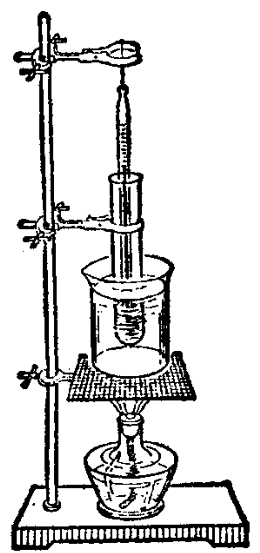
\includegraphics[width=4cm]{../pic/czwl2-ch4-1}
    \caption{观察萘的熔解}\label{fig:4-1}
\end{wrapfigure}

这一节我们来研究物质从固态变成液态或者由液态变成固态的规律。
物质从固态变成液态,叫做\textbf{熔解};
    从液态变成固态,叫做\textbf{凝固}。
现在用实验来研究熔解和凝固的过程。

\xiaobiaoti{熔点和凝固点}
把装有萘的试管放在盛有水的烧杯里,在试管中插入温度计,用酒精灯通过烧杯和水均匀地给萘加热(图 \ref{fig:4-1})。
萘吸收热量,温度不断升高,当温度上升到 80 ℃ 时,开始熔解。
在熔解过程中,虽然继续加热,但萘的温度却保持 80 ℃ 不变,直到完全熔解后,温度才继续上升。
这表明,萘是在一定的温度下熔解的。

把松香装在试管里,做同样的实验,可以看出,固态的松香先是变软,然后逐渐变成液态。
松香在整个熔解过程中,温度不断上升,并不保持一定的温度。
可见,松香没有一定的熔解温度。

固体分晶体和非晶体两类。
萘、冰、石英、水晶、食盐、海波、各种金属、大多数矿石都是晶体。
松香、玻璃、蜂蜡、沥青等都是非晶体。

实验表明,
所有的晶体都跟萘一样,在一定的温度下熔解;
所有的非晶体都跟松香一样,没有一定的熔解温度。

晶体熔解时的温度叫做\textbf{熔点}。晶体不同,熔点也不同。

\begin{table}[H]
    \centering
    \caption*{几种物质的熔点(℃)}
    \begin{tblr}{
        colspec={|ll|ll|ll|},
        columns={colsep+=0.5em},
        column{6}={mode=math},
    }
        \hline
        钨 & 3410 & 铝 & 660 & 固态水银 & -39 \\
        纯铁 & 1535 & 铅 & 327 & 固态酒精 & -117 \\
        钢 & 1130~1400 & 锡 & 232 & 固态氮 & -210 \\
        铸铁 & 约 1200 & 萘 & 80 & 固态氢 & -259 \\
        铜 & 1083 & 海波 & 48 & 固态氨 & -272 \\
        金 & 1064 & 冰 & 0 &  &  \\
        \hline
    \end{tblr}
\end{table}


在图 \ref{fig:4-1} 所示的实验中,在萘熔解成液体以后,如果停止对烧杯加热,液态萘的温度就不断降低。
当温度降到 80 ℃ 时,萘开始凝固。萘在凝固过程中,温度保持不变,直到全部凝固后,温度才又开始下降。
可见,晶体不但在一定的温度下熔解,也在一定的温度下凝固。
晶体凝固时的温度叫做\textbf{凝固点}。同一物质的凝固点跟它的熔点相同。


\begin{figure}[htbp]
    \centering
    %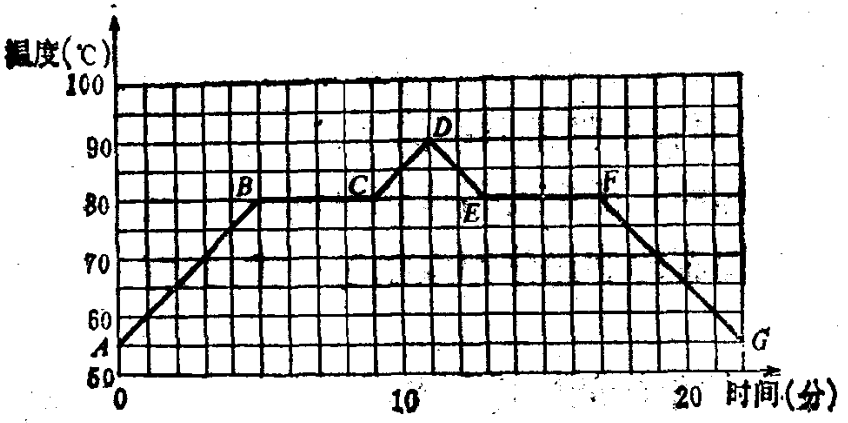
\includegraphics[width=0.6\textwidth]{../pic/czwl2-ch4-2.old}
    \begin{tikzpicture}[>=Stealth, scale=0.8]
    \draw [thick,->] (0, 0) -- (12, 0) node[anchor=north] {时间(分)};
    \draw [thick,->] (0, 0) -- (0, 6) node[anchor=east] {温度(℃)};

    \foreach \x in {0.5, 1, 1.5, ..., 11} {
        \draw (\x, 0) -- (\x, 5);
    }

    \foreach \y in {0.5, 1, 1.5, ..., 5} {
        \draw (0, \y) -- (11, \y);
    }

    \foreach \x in {0,10,20} {
        \draw (\x/2,0.2) -- (\x/2,0) node[anchor=north] {$\x$};
    }
    \foreach \y in {50,60,...,100} {
        \tikzmath{
            \v = (\y-50)/10;
        }
        \draw (0.2,\v) -- (0,\v) node[anchor=east] {$\y$};
    }

    \coordinate (A) at (0, 0.5);
    \coordinate (B) at (2.5, 3);
    \coordinate (C) at (4.5, 3);
    \coordinate (D) at (5.5, 4);
    \coordinate (E) at (6.5, 3);
    \coordinate (F) at (8.5, 3);
    \coordinate (G) at (11, 0.5);

    \draw [very thick] (A) -- (B) -- (C) -- (D) -- (E) -- (F) -- (G);
    \foreach \n/\x/\y in {
            A/-0.3/0, B/-0.3/0.3, C/-0.3/0.3, D/0.3/0.3,
            E/-0.3/-0.3, F/0.3/0.3, G/0.3/0} {
        \coordinate (P) at (\x, \y);
        \node [fill=white, inner sep=0pt, font=\footnotesize] at ($(P) + (\n)$) {$\n$};
        \draw [fill=black] (\n) circle (2pt);
    }
\end{tikzpicture}

    \caption{萘的熔解和凝固图象}\label{fig:4-2}
\end{figure}

\xiaobiaoti{熔解和凝固图象}
物质的熔解和凝固过程,可以用图象来表示。图 \ref{fig:4-2}\footnotemark 是萘的熔解和凝固图象。
\footnotetext{注:原书的图模糊不清,我使用 tikz 绘制了一个图片。} % 原书图片 保存为 pic 目录下的 czwl2-ch4-2.old.png
图中,横坐标表示时间,纵坐标表示温度,从萘的温度是 55 ℃ 开始计时,
图象 $ABCDEFG$ 表示了萘在加热和冷却程中,它的温度随时间而变化的情况。
其中,$BC$ 部分表示萘的熔解过程,$EF$ 部分表示疑固过程。
从图中可以看出,萘在熔解和凝固过程中温度保持不变,它的熔点和凝固点都是 80 ℃。
象这样用图象来表示物理量的变化情况,是物理学中常用的方法。
在物理实验中,就常常用图象把实验结果表示出来,它能直观地表示出物理量的变化规律。


\xiaobiaoti{熔解热}
晶体在熔解过程中虽然温度保持不变,但要继续给它加热,熔解过程才能完成。
这表明晶体在熔解过程中要吸收热量。
单位质量的某种晶体,在熔点变成同温度的液体时吸收的热量,叫做这种物质的\textbf{熔解热}。
液体在凝固时要放出热量。
单位质量的液体,在凝固点变成同温度的晶体时放出的热量,等于它的熔解热。
例如,冰的熔解热是 80 卡/克, 1 克水在 0 ℃ 疑固成 0 ℃ 的冰放出的热量也是 80 卡。



\lianxi

(1) 在很冷的地区,为什么不用水银温度计而用酒精温度计来测量气温?

(2) 要使热的物体冷却,用质量相等的 0 ℃ 的水或 0 ℃ 的冰,哪一种效果好些?为什么?

(3) 把正在熔解的冰拿到 0 ℃ 的房间里,冰能不能继续熔解?为什么?
把装在瓶里的水放在 0 ℃ 的房间里,水能不能结冰?为什么?

(4) 电灯泡发光时灯丝的温度达到 2000 ℃。能用铁、金、铅来制造电灯泡的灯丝吗?
如果由你来挑选,你准备选哪种金属来制造电灯泡的灯丝?说明你的理由。



\section{实验:研究萘的熔解过程}\label{sec:4-2}

这个实验是要研究萘受热熔解时,它的温度变化情况。

把萘粉装进试管,试管里插入温度计和搅动器,温度计的玻璃泡要插进萘粉中。
把试管放到盛有热水的烧杯里,用酒精灯给烧杯缓缓加热,同时用搅动器搅动萘粉,
使萘的各部分温度均匀。实验装置跟图 \ref{fig:4-1} 一样。

观察温度计的示数,等萘的温度升到 50 ℃ 左右,开始每隔一分钟或两分钟记录一次萘的温度。
直到萘的温度大约升到 85 ℃ 为止。把实验数据记录在表格里。

\jiange
\begin{tblr}{
    hlines,
    colspec={|c|*{7}{c}c|},
    column{2-8} = {wd=2em},
}
    时间(分) & 0, & 1, & 2, & 3, & 4, & 5, & 6, & …… \\
    温度(℃) & & & & & & & & \\
\end{tblr}
\jiange

以横坐标表示时间,以纵坐标表示温度,在方格纸上标出一些点,用来表示实验得到的萘在各个时刻的温度。
用平滑的曲线把这些点连接起来,就得到了萘的熔解图象。从你画的图象中,得出萘的熔点是多少度?

如果有时间的话,还可以做萘的凝固图象。看看你得出的萘的凝固点跟它的熔点是否相同?


\section{汽化}\label{sec:4-3}

物质从液态变成气态的现象叫做\textbf{汽化}。汽化有两种方式:蒸发和沸腾。

\xiaobiaoti{蒸发}
我们知道,洗过的湿衣服,能晒干也能晾干。
放在敞口容器里的水,过些天会变少。
往碟子里倒一点酒精,很快就干了,并且满屋子都能闻到酒精的气味。
这几个例子里液体都变成了气体,汽化了。
这些汽化现象都是从液体的表面发生的。
只从液体表面发生的汽化现象叫做\textbf{蒸发}。

同样湿的衣服,夏天干得快,冬天干得慢。
这表明液体的温度越高,蒸发得越快。

同样多的水,倒在碟子里干得快,装在瓶子里干得慢。
这表明液体的表面积越大,蒸发得越快。

同样湿的衣服挂在有风的地方干得快,挂在没有风的地方干得慢。
这表明液体表面上的空气流动得越快,蒸发得越快。

可见,为了加快液体蒸发,可以提高液体的温度,增大液体的表面积和加快液体表面上的空气流动。

液体蒸发时还产生一种现象,就是液体的温度降低。这可以从下述的实验看出。
拿两支温度计,用棉花把一支温度计的泡包上,并用温度跟室温相同的酒精把棉花浸湿。
这时棉花上的酒精在蒸发,我们看到,带着湿棉花的温度计表示的温度比另一支温度计的低〈图 \ref{fig:4-3})。

\begin{figure}[htbp]
    \centering
    \begin{minipage}{7cm}
    \centering
    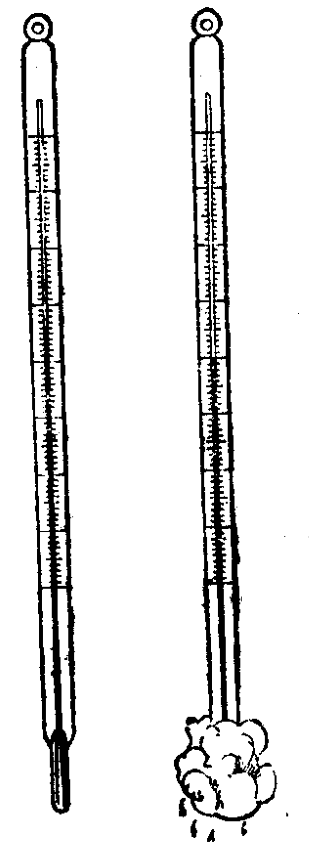
\includegraphics[width=3cm]{../pic/czwl2-ch4-3}
    \caption{液体蒸发时温度降低}\label{fig:4-3}
    \end{minipage}
    \qquad
    \begin{minipage}{7cm}
    \centering
    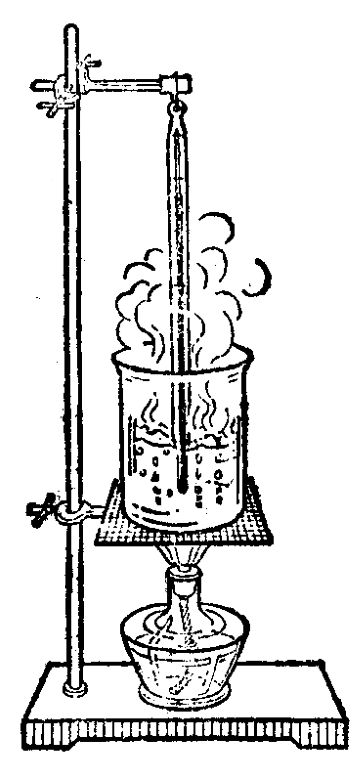
\includegraphics[width=4cm]{../pic/czwl2-ch4-4}
    \caption{水的沸腾}\label{fig:4-4}
    \end{minipage}
\end{figure}

液体蒸发时温度降低,说明它要从周围的物体吸收热量,因此液体蒸发有致冷作用。
在皮肤上擦一点酒精或水,就会感到凉,这是因为酒精或水蒸发时,从身体吸收了热量,使皮肤的温度降低了的缘故。




\xiaobiaoti{沸腾}
把水放在烧杯里加热,当温度升到一定程度时,水中就会发生剧烈的汽化现象,形成大量的汽泡,
上升到水面破裂开来,把里面的水蒸气放掉(图 \ref{fig:4-4}),这种现象叫做\textbf{沸腾}。

蒸发和沸腾这两种汽化现象是有区别的。
蒸发是只在液体表面发生的汽化现象,
沸腾是在液体内部和表面上同时发生的剧烈的汽化现象。

\begin{wrapfigure}{r}{6cm}
    \centering
    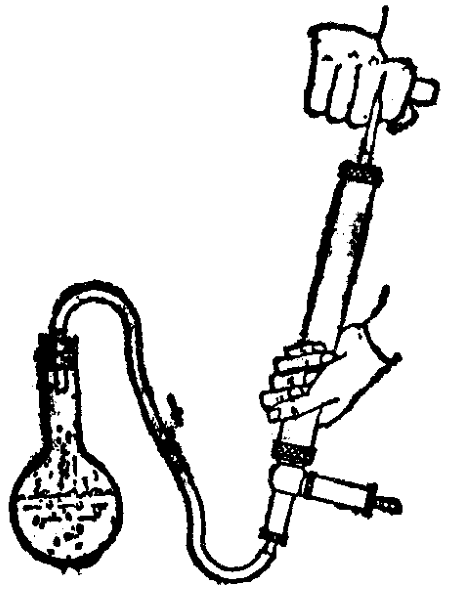
\includegraphics[width=5cm]{../pic/czwl2-ch4-5}
    \caption{水在低压下沸腾}\label{fig:4-5}
\end{wrapfigure}

在图 \ref{fig:4-4} 的实验里,把温度计插入水里来观察水在沸腾时的温度,可以看到水在沸腾过程中,
虽然对它继续加热,它的温度却保持不变。这表明液体是在一定的温度下沸腾的。
沸腾只在一定温度下发生,而蒸发在任何温度下都能发生,这也是它们的区别。

液体沸腾时的温度叫做\textbf{沸点}。不同的液体沸点不同。
即使同一种液体,它的沸点也要随液面上的气压而改变。
在瓶里装入低于 100 ℃ 的水,抽出瓶里的空气,使气压降低,
就会看到水也会沸腾起来(图 \ref{fig:4-5})。
这表明,在压强减小的时候,液体的沸点降低。
相反,如果增加压强,液体的沸点就要升高。

可见,液体的沸点跟压强有关系。
压强增大,沸点升高;
压强减小,沸点降低。

液体的沸点随压强而改变的现象有许多实际应用。
在火力发电厂的锅炉里,要在高压下给水加热,使水的沸点升高,以便得到高温高压的水蒸气。
日常生活里用的高压锅,也是利用高压下沸点升高的道理来更快地煮熟饭菜的。


\begin{table}[H]
    \centering
    \caption*{几种液体在1 标准大气压下的沸点(℃)}
    \begin{tblr}{
        colspec={|ll|ll|ll|},
        columns={colsep+=0.5em},
        column{2,4,6}={mode=math},
    }
        \hline
        液态铁 & 2750 & 水 & 100 & 液态氧 & -183 \\
        液态铅 & 1740 & 酒精 & 78 & 液态氮 & -196 \\
        水银 & 357 & 乙醚 & 35 & 液态氢 & -253 \\
        萘 & 218 & 液态氨 & -33 & 液态氦 & -268.9 \\
        \hline
    \end{tblr}
\end{table}


\xiaobiaoti{汽化热}
液体蒸发时要吸收热量。液体在沸腾过程中,虽然对它继续加热,
但是它的温度保持不变,这就是说液体沸腾时也要吸收热量。
单位质量的某种液体变成同温度的气体时吸收的热量,叫做这种液体的\textbf{汽化热}。
例如,水的汽化热在 100 ℃ 时是 539 卡/克,
即 1 克 100 ℃ 的水变成 100 ℃ 的水蒸气吸收 539 卡的热量。



\lianxi

(1) 晒粮食时,为什么要把粮食放在向阳的地方,并把粮食摊开?

(2) 在刮风时,土地容易变干,但塑料大棚里的土地不容易变干。为什么?

(3) 夏天扇扇子,空气的温度并没有降低,为什么会感到凉爽些?

(4) 有一种粘木料用的胶,需要在 100 ℃ 左右的温度下熬化后才能使用,温度再高就会熬焦,失去粘性。
所以熬这种胶最好用图 \ref{fig:4-6} 所示的两层锅,两层锅之间装着水,这样就不会把胶熬焦了,为什么?

(5) 在高山上用普通的锅煮鸡蛋,水烧开很久,鸡蛋也煮不熟,为什么?怎样才能把鸡蛋煮熟?

(6) 在制糖工业中,要用沸腾的办法除去糖汁中的水分。
为了使糖在沸腾的时候不致变质,沸腾的温度要低于100 ℃ 。想想看,怎样可以做到这一点。

(7) 火箭在大气中飞行时,它的头部跟空气摩擦而产生大量的热,会因温度过高而烧坏。
在火箭头部涂上一层特殊材料,这种材料在高温下熔解并汽化,就能起到保护火箭头部的作用,为什么?


\begin{figure}[htbp]
    \centering
    \begin{minipage}{7cm}
    \centering
    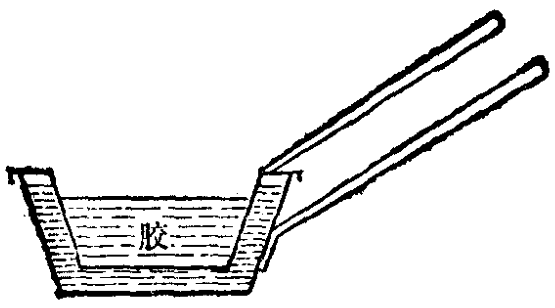
\includegraphics[width=6cm]{../pic/czwl2-ch4-6}
    \caption{熬胶锅}\label{fig:4-6}
    \end{minipage}
    \qquad
    \begin{minipage}{7cm}
    \centering
    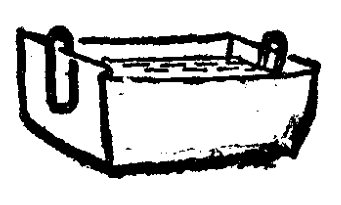
\includegraphics[width=5cm]{../pic/czwl2-ch4-7}
    \caption{烧开水用的纸盒}\label{fig:4-7}
    \end{minipage}
\end{figure}


\section*{小实验}

你相信能用纸盒把水烧开吗?

用一张表面光滑的厚纸做成一个小纸盒,用曲别针把它夹住(图 \ref{fig:4-7})。
纸盒里装些水,放到火上加热。
注意不要让火苗烧到水面以上的纸盒,过一会水就会沸腾起来,而纸盒不会烧着。

你实际做一做,并说明为什么纸盒不会烧着。


\section{液化}\label{sec:4-4}

物质从气态变成液态的现象叫做\textbf{液化}。
正象凝固是熔解的相反过程一样,液化是汽化的相反过程.

\begin{wrapfigure}{r}{7cm}
    \centering
    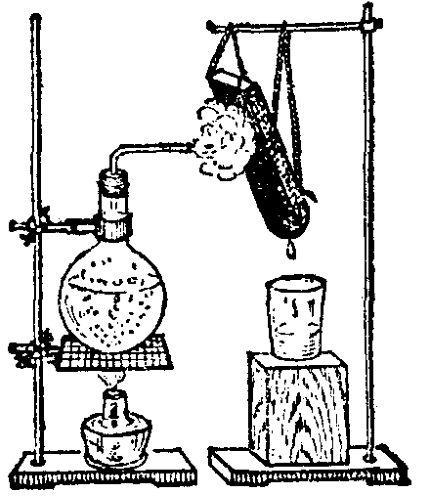
\includegraphics[width=6cm]{../pic/czwl2-ch4-8}
    \caption{水蒸气温度降低凝结成水}\label{fig:4-8}
\end{wrapfigure}


让水蒸气喷到一个冷的物体上,水蒸气就变成水(图 \ref{fig:4-8})。
烧水时看到的“白气” 就是水蒸气温度降低凝结成的小水珠。
可见,降低温度,可以使水蒸气液化。

实验表明,所有的气体,在温度降低到足够低的时候,都可以液化。

气体的液化温度跟压强有关系。
例如,水蒸气在 1 标准大气压下,液化温度是 100 ℃;
在 3 标准大气压下,要在 134 ℃ 才凝结成水。
可见,气体的压强越大,它的液化温度越高。

一些通常情况下是气体状态的物质,在大气压下要在很低的温度才能液化;
如果采用增大压强的办法,在较高的温度下就可以使它们液化。
例如,许多地方使用的液化石油气,就是在常温下用增大压强的方法,
使它成为液体储存在钢罐里的。

跟液体在汽化时要吸收热量相反,气体在液化时要放出热量。
被水蒸气烫伤往往比被开水烫伤还严重,就是因为水蒸气液化时放出了热量的缘故。

实验表明,某种物质在从气体变成同温度的液体时放出的热量,
等于它在这一温度下,由液体变成气体时吸收的热量。
这就是说,单位质量的某种物质,在从气体变成同温度的液体时放出的热量,
等于它在这一温度时的汽化热。
例如,1 克 100 ℃ 的水蒸气在凝结成 100 ℃ 的水时,放出的热量就是 539 卡。

在自然界中,我们可以看到水蒸气凝结成水的例子。
白天气温较高,地球表面的水大量蒸发,空气中有较多的水蒸气;
夜间气温较低,空气中的水蒸气就在草木、石块等上面凝成小水珠,这就是露。
如果空气中有较多的浮尘,空气中的水蒸气就凝结在这些浮尘上面,这就是雾。


\section*{阅读材料:致冷设备}

我们知道,液体汽化时有致冷作用,致冷设备就是根据这种作用制成的。

常用的致冷设备主要由压气机、冷凝器和蒸发器三部分组成(图 \ref{fig:4-9})。
\begin{figure}[htbp]
    \centering
    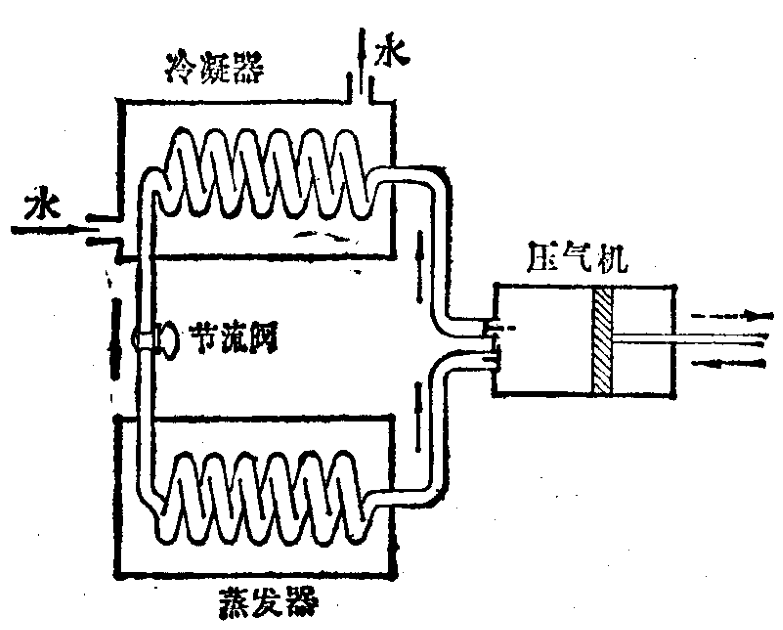
\includegraphics[width=0.6\textwidth]{../pic/czwl2-ch4-9}
    \caption{致冷设备的示意图}\label{fig:4-9}
\end{figure}
其中的工作物质是容易由气态变成液态和由液态变成气态的物质,常用的有氨及氟氯烷等。
压气机产生大约 10 标准大气压的压强,把气态氨压入冷凝器的管里,这时氨变了液体。
氨在液化时放出的热量被流动的冷水吸收并带走。
冷凝器的管里的液态氨通过节流阀缓慢地进入蒸发器的管里。
由于压气机不断地从蒸发器的管里吸走气体,这个管里的压强就比较低,于是液态氨在蒸发器的管里迅速汽化。
在汽化中从管外的食盐水里吸取热量,使食盐水的温度降低。
生成的氨气又被压气机抽走,压入冷凝器,这样氨可以循环使用。
温度降低后的食盐水可作为致冷剂用来制冰、冷却食品或降低夏季房间里的气温。
在用于降低房间里的气温时,通常不用食盐水而是直接使空气从蒸发器管子的周围流过而得到冷却,
再把冷却后的空气送到房间里去。



\section{升华和凝华}\label{sec:4-5}

物质不但可以在固态和液态之间,或者在液态和气态之间进行变化,也可以直接在固态和气态之间进行变化。
物质从固态直接变成气态叫做\textbf{升华},从气态直接变成固态叫做\textbf{凝华}。

升华和凝华的现象是经常可以遇到的。
冬天,晾在室外的湿衣服里的水会结成冰,但冰冻的湿衣服也会干,就是因为冰直接变成了水蒸气。
在冬天的早晨,我们常常看到霜。霜就是空气中的水蒸气直接凝华而成的。

用固态的碘很容易看到升华和凝华现象。
把少量的碘放进烧瓶里,微微加热,固态的碘就升华,产生紫色的碘蒸气。
停止加热后,会在烧瓶壁上看到疑华成的固态碘。
用久了的电灯泡会发黑,是因为钨丝受热产生升华现象,然后钨的气体又在灯泡壁上凝华的缘故。

空气里总是含有水蒸气的。
当含有很多水蒸气的空气升入高空时,水蒸气温度降低就要疑结成小水滴或凝华成小冰晶。
天空中的云就是由大量的小水滴和小冰晶形成的。
在一定条件下,小水滴和小冰晶越来越大,达到一定程度时就会下落。
在下落过程中冰晶熔解成水滴,与原来的水滴一起落到地面,这就形成了雨。

物质在升华过程中要吸收热量,在凝华过程中要放出热量。
生产中可利用升华吸热的现象来取得低温。
例如,在实验室里,常用固态二氧化碳(干冰)的升华吸热来获得低温。



\lianxi

(1) 冬天可以看到呼出的“ 白气” ,而在夏天却看不见,为什么?

(2) 在北方的冬天,戴眼镜的人从外面进到嗳和的屋子里,镜片上会出现一层小水珠,为什么?

(3) 夏天在箱子里放些卫生球(用萘制的),用来预防虫蛀,过几个月后再看,卫生球变小或消失了。解释这个现象。

(4) 在很冷的冬夜里,房间门窗玻璃的内表面往往结一层冰花。试说明冰花是怎样产生的。


\section*{复习题}

(1) 什么叫熔解?什么叫凝固?什么叫熔点?什么叫疑固点?晶体和非晶体的熔解和凝固有什么区别?

(2) 什么叫蒸发?蒸发的快慢跟哪些因素有关系?

(3) 什么叫沸腾?沸腾跟蒸发有什么不同?什么叫沸点?液体的沸点跟压强有什么关系?

(4) 什么叫液化?气体的液化温度跟压强有什么关系?

(5) 什么叫升华?什么叫凝华?

(6) 在熔解、凝固、汽化、液化、升华、凝华中,哪些过程吸收热量,哪些过程放出热量?什么叫熔解热?什么叫汽化热?



